\subsection{Merancang Arsitektur dan Desain Integrasi Sistem}
\label{subsec:merancang-aristektur-dan-desain-integrasi-sistem}

Subbab ini menjelaskan mengenai struktur dan organisasi sistem yang akan dibangun dari berbagai pandangan arsitektur yang digunakan untuk menggambarkan sistem. Rancangan sistem dibuat dengan mengacu pada kebutuhan fungsional dan nonfungsional yang telah 
dianalisis sebelumnya, untuk memastikan sistem yang dikembangkan memenuhi tujuan dan kebutuhan pengguna.

Pendekatan yang digunakan untuk membuat desain arsitektur ini adalah 4+1 View Model. Model ini mengorganisasikan arsitektur sistem ke dalam lima pandangan yang berbeda, yaitu \emph{scenarios view}, \emph{logical view}, \emph{process view}, \emph{development view}, dan \emph{physical view}. Setiap pandangan memberikan perspektif yang berbeda terhadap sistem sehingga dapat memberikan gambaran yang komprehensif mengenai arsitektur sistem yang akan dibangun. Pendekatan ini memungkinkan proses pengembangan sistem menjadi lebih terstruktur dan sistematis.

\subsubsection{\emph{Scenarios View}}
\label{subsubsec:use-case-view}

\emph{Scenarios View} menunjukkan perilaku sistem dari sudut pandang pengguna melalui pemodelan \emph{use case}. \autoref{fig:bpmn-to-be} menunjukkan \emph{Business Process Model and Notation} (BPMN) untuk \emph{use case} utama sistem, yaitu \emph{share-extract-save}. BPMN ini menunjukkan perbedaan alur kerja dari BPMN sistem saat ini (\emph{As-Is}) yang telah ditunjukkan pada \autoref{sec:analisis-kondisi-saat-ini}. Proses manual yang perlu dilakukan pengguna mulai dari mengekstrak data hingga menyimpan hasil pencatatan pengeluaran ke dalam aplikasi telah diotomatisasi pada sistem yang diusulkan.

\autoref{fig:use-case-diagram} menunjukkan \emph{use case diagram} sistem pencatatan pengeluaran berbasis \emph{mobile}. Diagram ini menggambarkan interaksi antara pengguna dan sistem pada \emph{use case} yang telah diidentifikasikan dari kebutuhan fungsional. \autoref{tab:use-case-list} menyajikan daftar \emph{use case} yang diidentifikasi dalam sistem beserta kode kebutuhan fungsional yang terkait.

\begin{figure}[htbp]
    \centering
    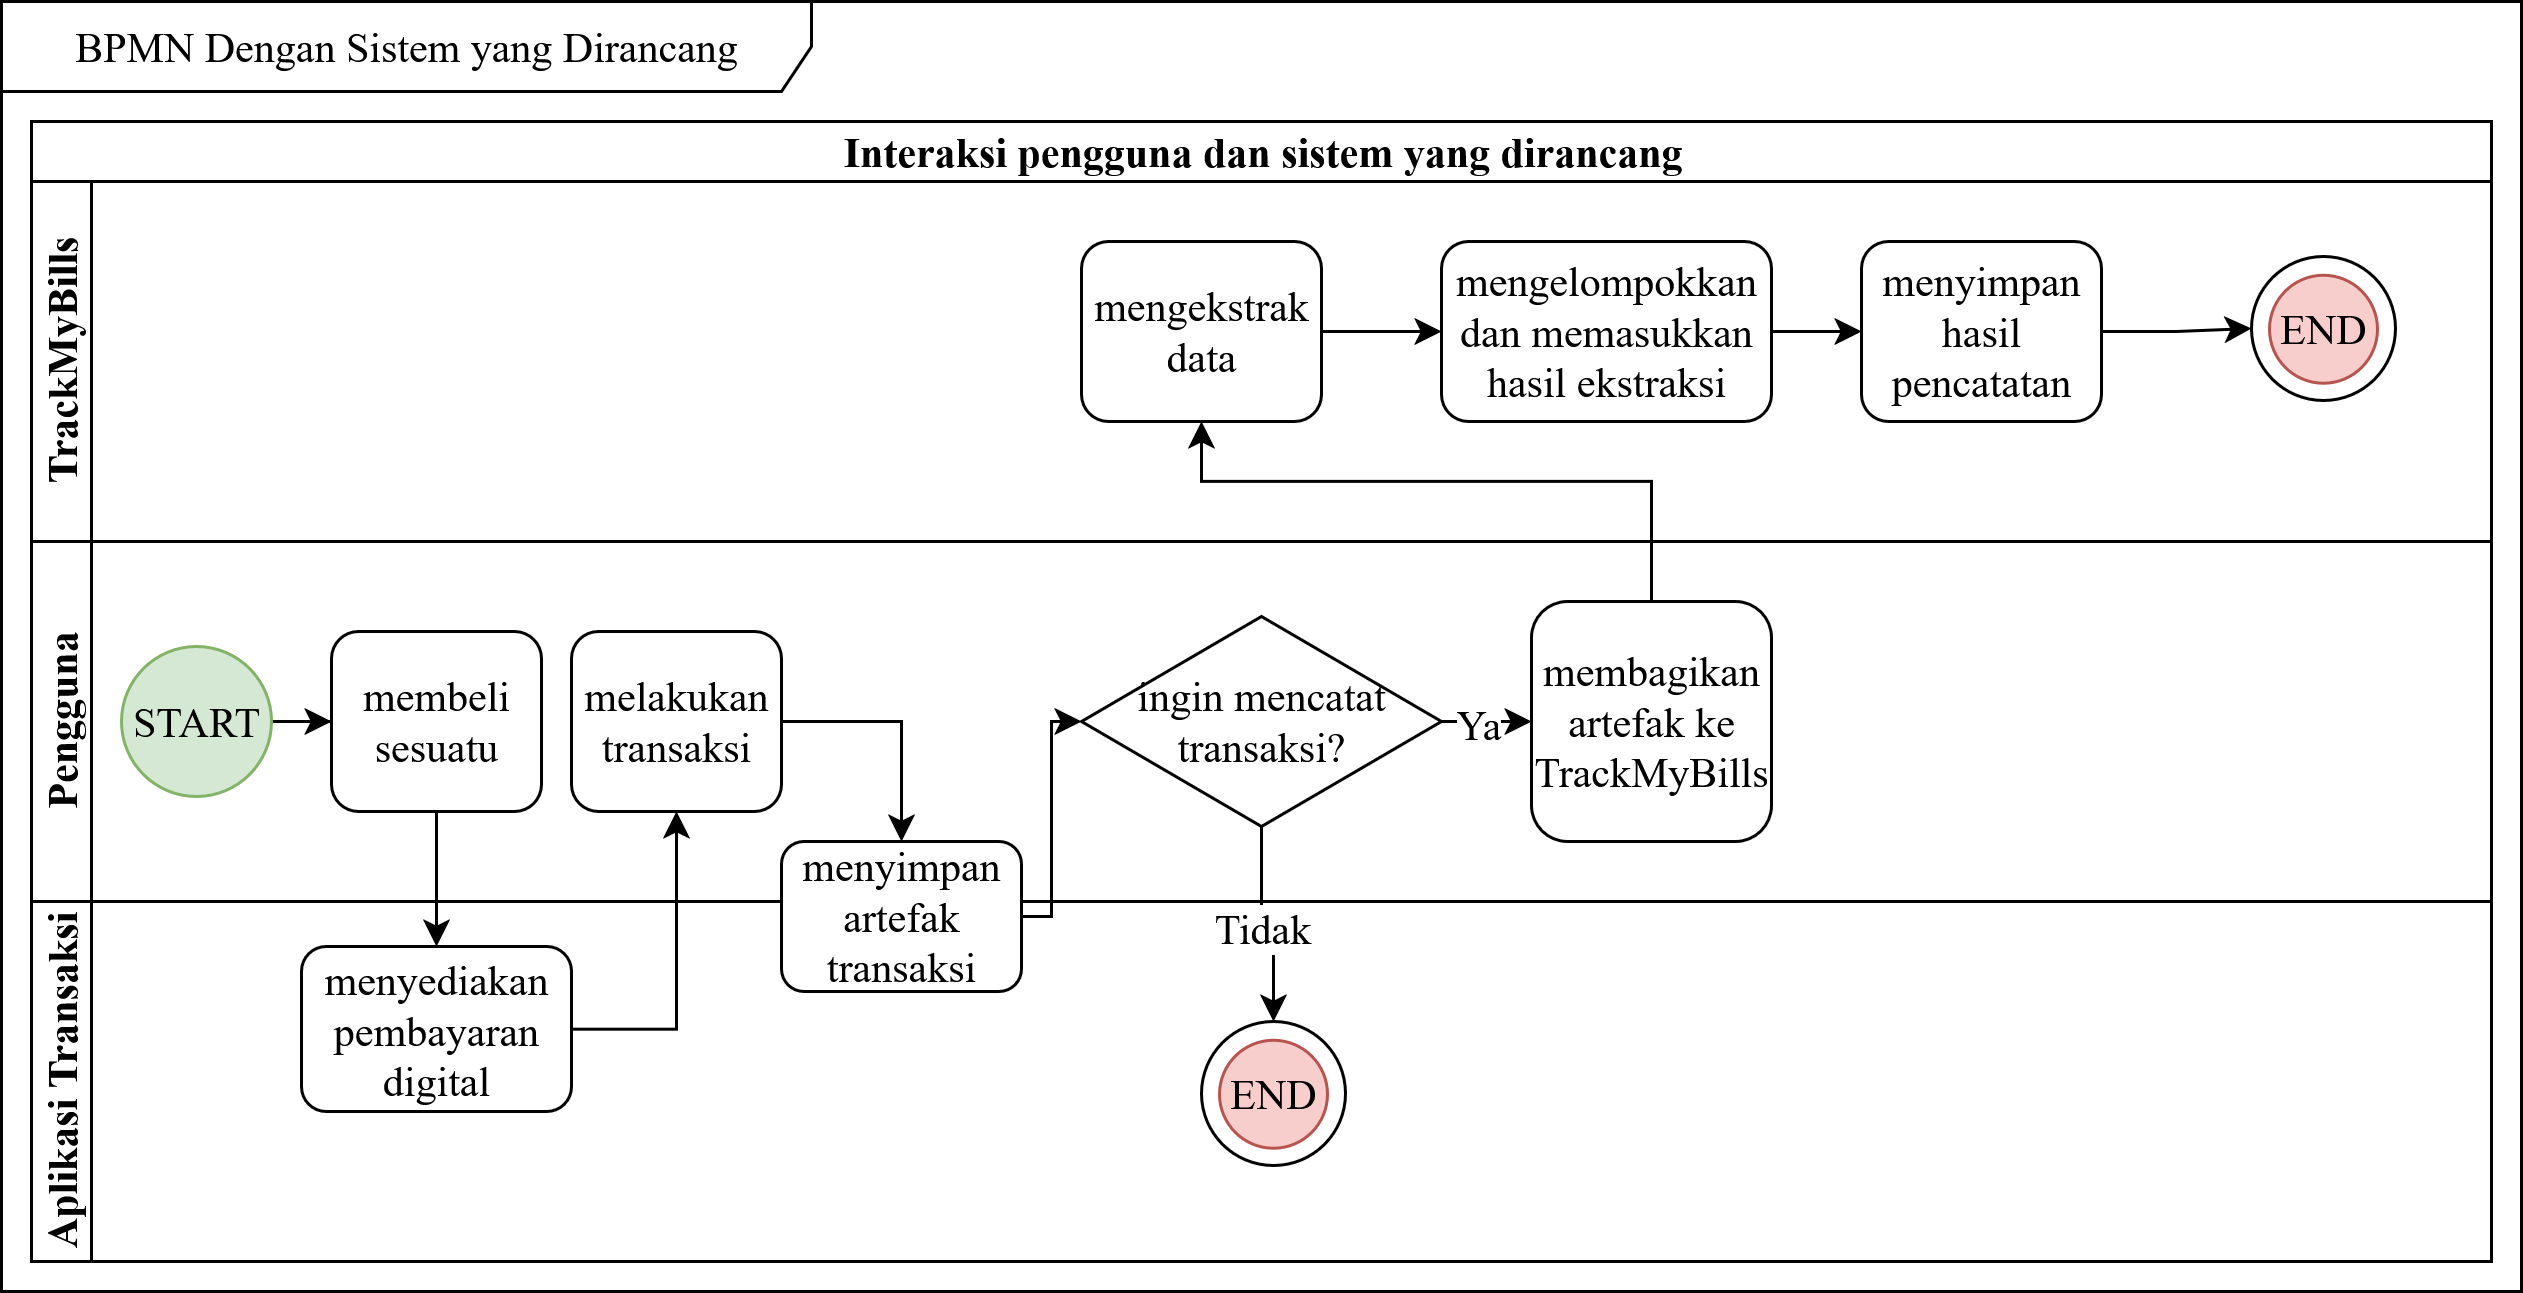
\includegraphics[width=1\textwidth]{images/To-be.png}
    \caption{BPMN untuk \emph{use case} utama sistem (\emph{share-extract-save})}
    \label{fig:bpmn-to-be}
\end{figure}

\begin{figure}[htbp]
    \centering
    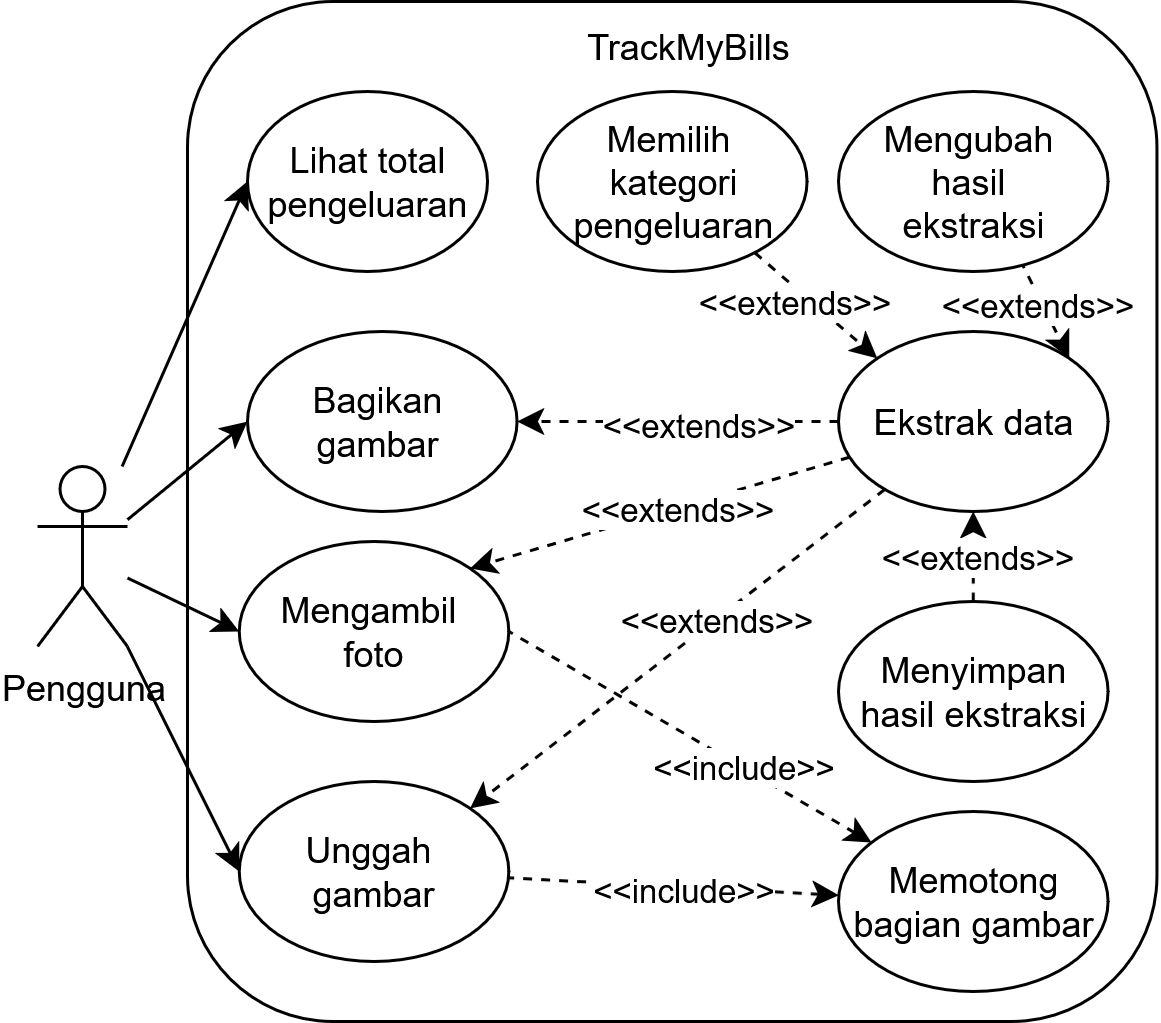
\includegraphics[width=.6\textwidth]{images/use-case-diagram.png}
    \caption{\emph{Use case diagram} sistem pencatatan pengeluaran berbasis \emph{mobile}}
    \label{fig:use-case-diagram}
\end{figure}

\begin{table}[h!]
\centering
\caption{Daftar \emph{use case} sistem pencatatan pengeluaran berbasis \emph{mobile}}
\label{tab:use-case-list}
\begin{tabularx}{\textwidth}{|p{1.6cm}|p{1.5cm}|p{2.8cm}|X|}
\hline
\textbf{Kode \emph{Use Case}} & \textbf{Kode FR} & \textbf{\emph{Use Case}} & \textbf{Deskripsi} \\ \hline
UC-01 & FR-01 & Bagikan gambar & Membagi (\emph{share}) gambar ke sistem \\ \hline
UC-02 & FR-01 & Mengambil foto & Mengakses kamera dari aplikasi dan mengambil foto \\ \hline
UC-03 & FR-01 & Unggah gambar & Memberikan izin mengakses foto dan mengunggah gambar dari galeri \\ \hline
UC-04 & FR-02 & Memotong bagian gambar & Memotong bagian gambar yang diperlukan \\ \hline
UC-05 & FR-03 & Ekstrak data & Mengekstrak data dari gambar yang telah diterima aplikasi \\ \hline
UC-06 & FR-04 & Memilih kategori pengeluaran & Memilih kategori dari data pengeluaran yang diekstrak \\ \hline
UC-07 & FR-04 & Mengubah hasil ekstraksi & Mengubah hasil ekstraksi data sebelum data disimpan \\ \hline
UC-08 & FR-05 & Menyimpan hasil ekstraksi & Menyimpan hasil ekstraksi data dari gambar yang diterima \\ \hline
UC-09 & FR-05 & Lihat total pengeluaran & Melihat total pengeluaran dan pengeluaran per kategori \\ \hline
\end{tabularx}
\end{table}

\subsubsection{\emph{Logical View}}
\label{subsubsec:logical-view}

\begin{figure}[htbp]
    \centering
    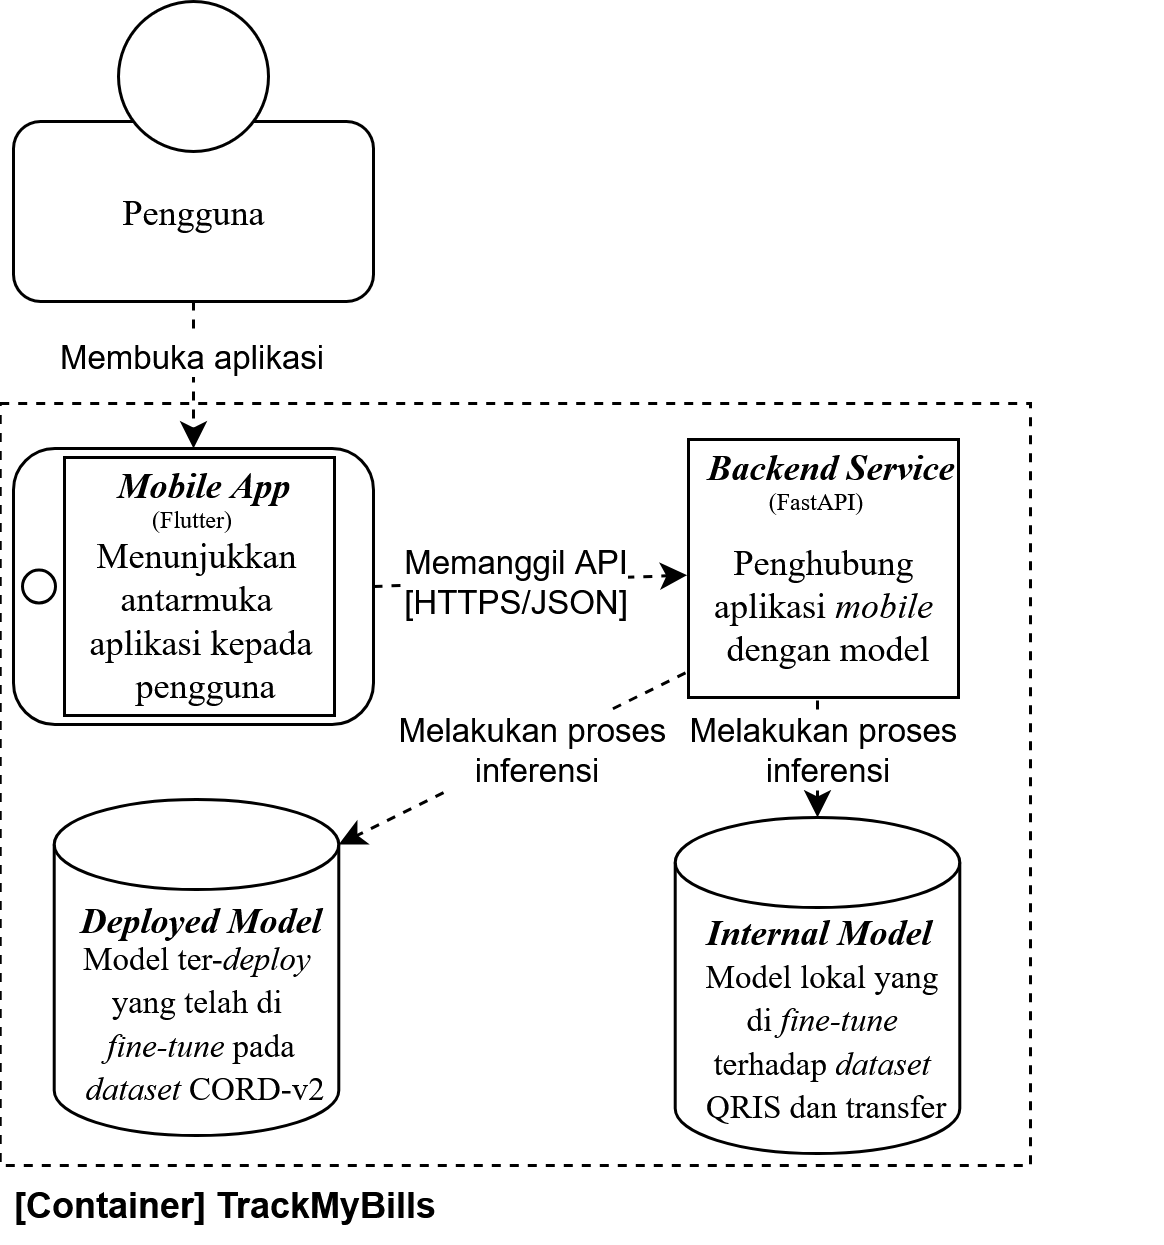
\includegraphics[width=.8\textwidth]{images/container-diagram.png}
    \caption{\emph{Container diagram} sistem pencatatan pengeluaran berbasis \emph{mobile}}
    \label{fig:container-diagram}
\end{figure}

\emph{Logical view} menggambarkan struktur sistem dari sudut pandang logis dari entitas-entitas yang ada dalam sistem secara konseptual. \autoref{fig:container-diagram} menunjukkan \emph{container diagram} sistem pencatatan pengeluaran berbasis \emph{mobile}. Diagram ini menunjukkan bagaimana sistem dibagi menjadi beberapa kontainer, yaitu aplikasi \emph{mobile}, layanan \emph{backend}, model internal, dan model \emph{deployed}. Setiap kontainer memiliki tanggung jawab dan interaksi yang jelas, yang memungkinkan pengembangan dan pemeliharaan sistem menjadi lebih terstruktur.

\autoref{fig:container-diagram} menunjukkan pengguna yang akan berinteraksi dengan aplikasi \emph{mobile}. Aplikasi \emph{mobile} berkomunikasi dengan layanan \emph{backend} melalui API, yang memungkinkan aplikasi untuk mengirim dan menerima data melalui protokol HTTP/JSON. Layanan \emph{backend} bertanggung jawab untuk memproses data dan menghubungkan dengan model internal dan model \emph{deployed}. Model internal dan model \emph{deployed} berfungsi untuk melakukan inferensi dari data yang diterima dari layanan \emph{backend}.




\subsubsection{\emph{Process View}}
\label{subsubsec:process-view}
\emph{Process view} menunjukkan alur kerja sistem dalam menangani proses bisnis dari perspektif interaksi antara pengguna dan sistem. \autoref{fig:activity-diagram} menunjukkan \emph{activity diagram} untuk proses \emph{share-extract-save} yang merupakan proses utama dari sistem yang dibangun. Sebelum proses dimulai, pengguna diasumsikan telah melakukan transaksi dan memiliki artefak transaksi berupa bukti pembayaran QRIS atau transfer. Proses dimulai dengan pengguna memiliki bukti pembayaran dan menggunakan fungsi \emph{share} yang disediakan sistem operasi untuk membagikan artefak tersebut ke aplikasi \emph{mobile}. Aplikasi \emph{mobile} akan menerima artefak tersebut dan menampilkan antarmuka untuk mengonfirmasi artefak yang ingin diproses. Jika artefak sesuai, aplikasi \emph{mobile} akan mengirim bukti pembayaran ke \emph{backend service} untuk divalidasi. Jika validasi berhasil, \emph{backend service} akan memproses bukti pembayaran dengan menggunakan model \donut{} untuk melakukan inferensi. Hasil inferensi akan diproses untuk menjadi format JSON yang sesuai dan dapat diterima aplikasi \emph{mobile}. Aplikasi \emph{mobile} menampilkan hasil pemrosesan untuk dikonfirmasi. Jika hasil telah sesuai dengan keinginan pengguna, pengguna dapat menyimpan hasil tersebut. Jika hasil pemrosesan masih belum sesuai dengan keinginan pengguna, pengguna masih dapat mengubah hasil ekstraksi dan kemudian menyimpan hasil yang telah diperbaiki.

\begin{figure}[htbp]
    \centering
    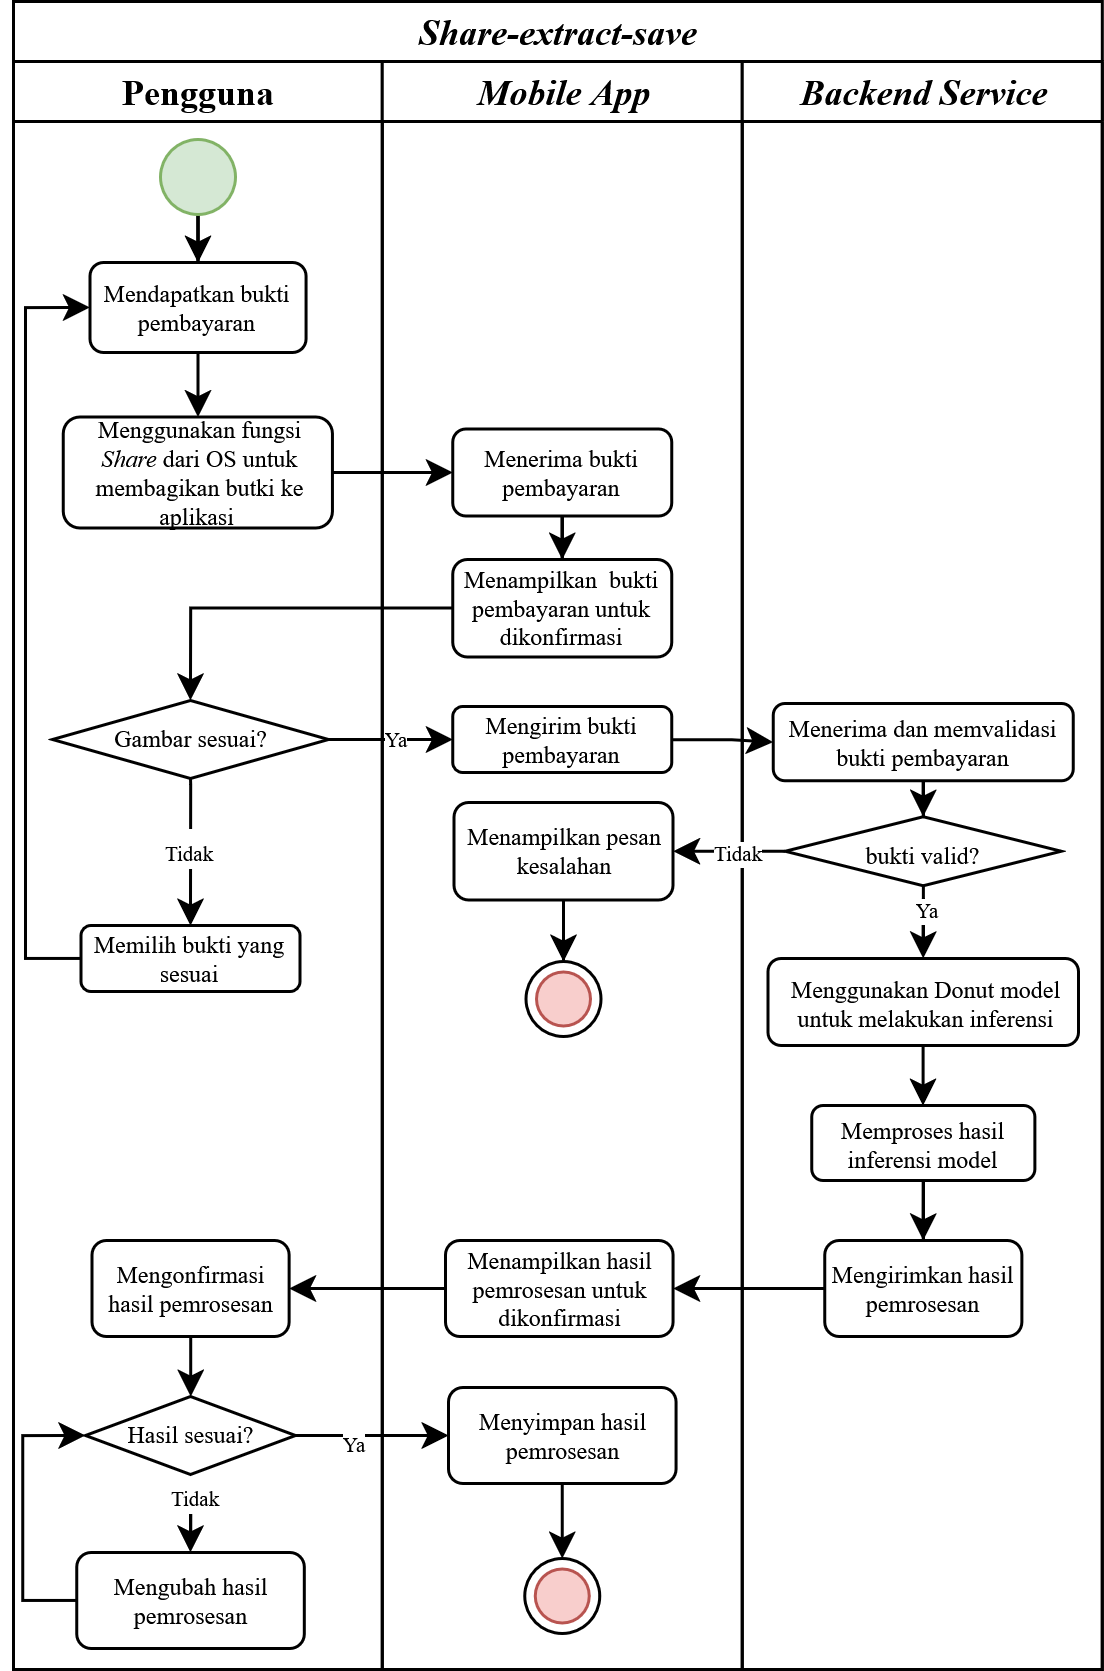
\includegraphics[width=.90625\textwidth]{images/activity-diagram.png}
    \caption{\emph{Activity diagram} untuk proses \emph{share-extract-save}}
    \label{fig:activity-diagram}
\end{figure}

\subsubsection{\emph{Physical View}}
\label{subsubsec:physical-view}
\emph{Physical view} menggambarkan bagaimana sistem dipetakan ke infrastruktur fisik, seperti jaringan, server, dan perangkat keras. \emph{Physical view} memastikan bahwa sistem dapat beroperasi dengan baik dalam lingkungan yang telah ditentukan. \autoref{fig:deployment-diagram} menunjukkan \emph{deployment diagram} sistem pencatatan pengeluaran berbasis \emph{mobile} yang menggambarkan aplikasi \emph{mobile}, layanan \emph{backend}, API \emph{Gateway} (ngrok \emph{tunnel}),model internal, dan model \emph{deployed}.
\begin{figure}[htbp]
    \centering
    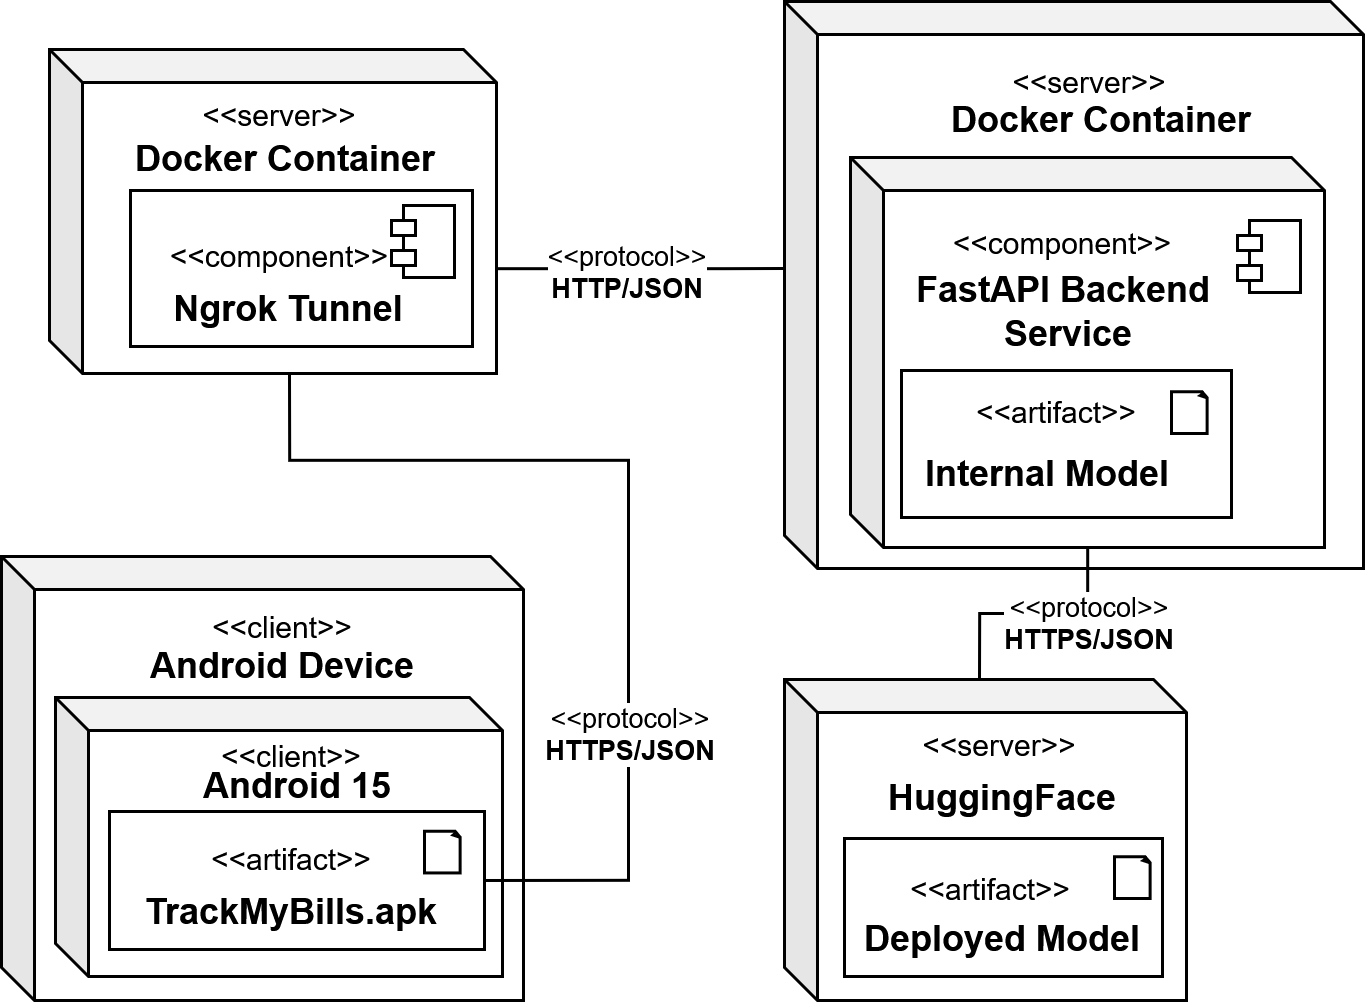
\includegraphics[width=1\textwidth]{images/deployment-diagram.png}
    \caption{\emph{Deployment diagram} sistem pencatatan pengeluaran berbasis \emph{mobile}}
    \label{fig:deployment-diagram}
\end{figure}

\subsubsection{\emph{Development View}}
\label{subsubsec:development-view}
\emph{Development view} mendefinisikan organisasi sistem dari sudut pandang pengembang. \emph{Development view} membuat pengembang dapat memahami struktur sistem hingga level komponen dan bagaimana komponen tersebut berinteraksi satu sama lain. \autoref{fig:component-diagram} menunjukkan \emph{component diagram} sistem pencatatan pengeluaran berbasis \emph{mobile}. Diagram ini menunjukkan bagaimana sistem dibagi menjadi beberapa komponen, yaitu aplikasi \emph{mobile}, layanan \emph{backend}, model internal, dan model \emph{deployed}. Setiap komponen memiliki tanggung jawab dan interaksi yang jelas dengan kompoenen lainnya untuk memungkinkan pengembangan sistem yang lebih terstruktur.

\begin{figure}[htbp]
    \centering
    % 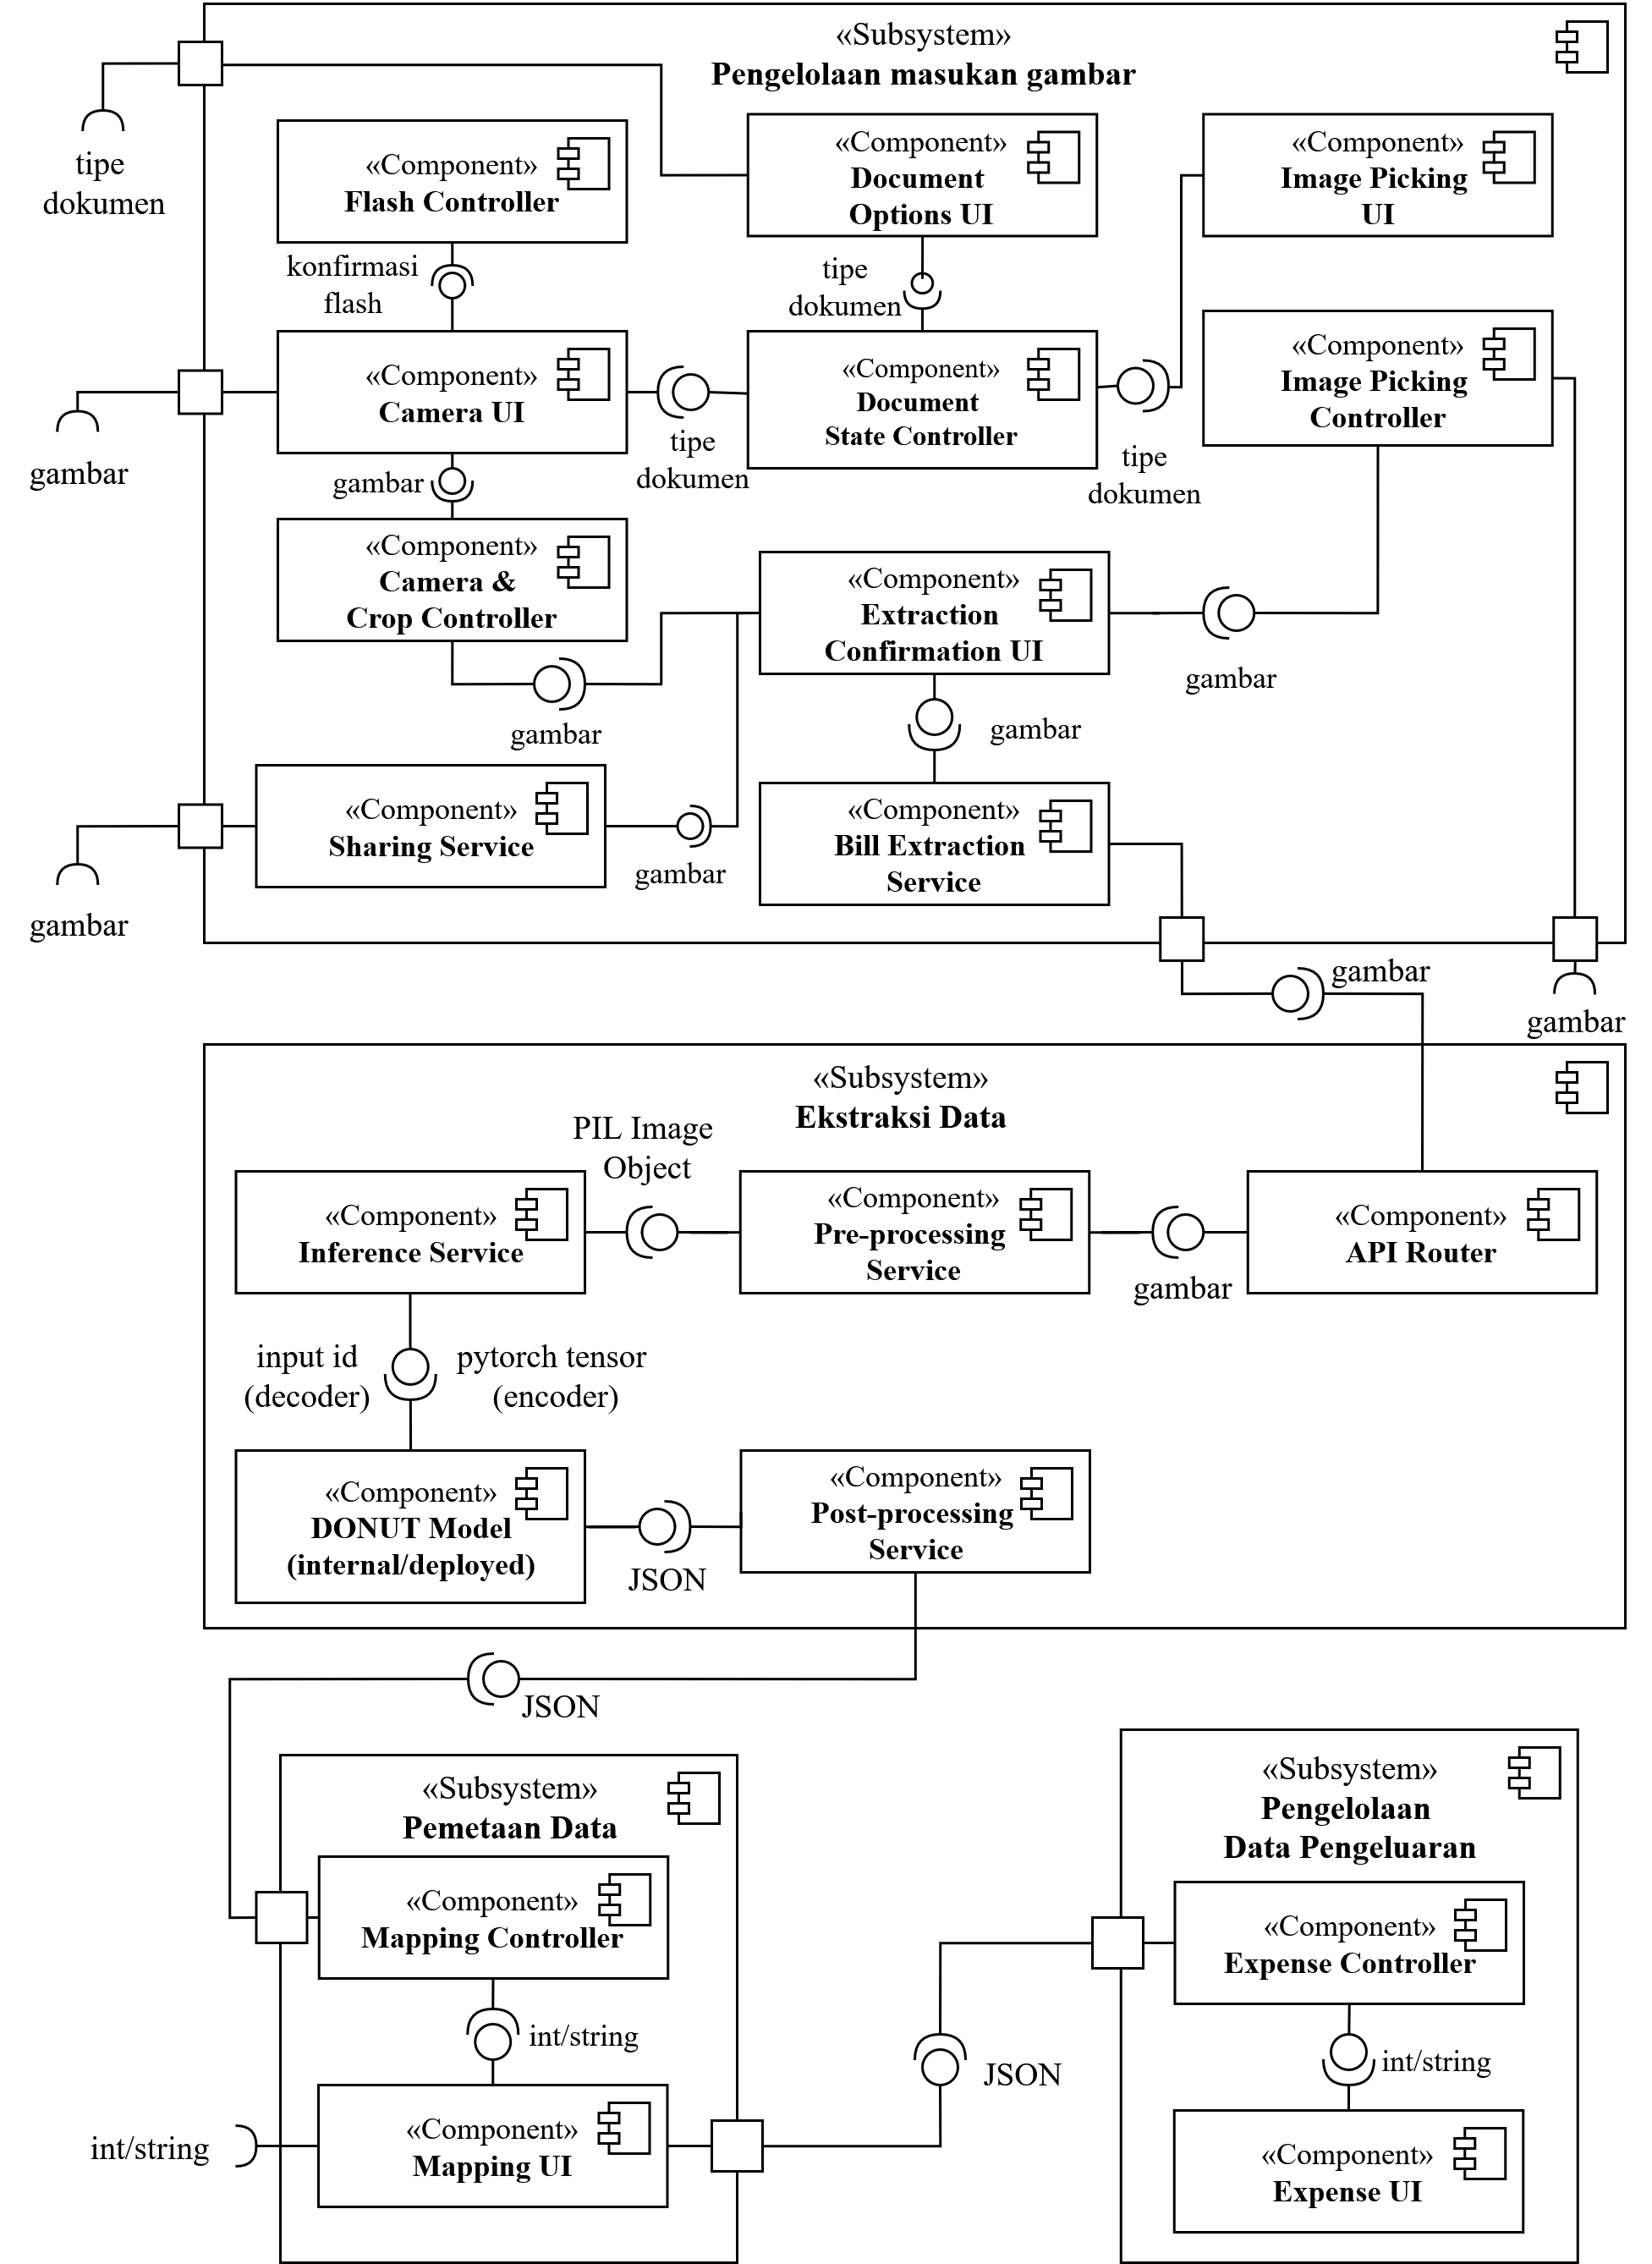
\includegraphics[width=1\textwidth]{images/component-diagram.png}
    \caption{\emph{Component diagram} sistem pencatatan pengeluaran berbasis \emph{mobile}}
    \label{fig:component-diagram}
\end{figure}